\subsubsubsection{Wavelet Network} \label{link::wavelet_nets}
\\\\
\indent Возвращаясь к частотно---временному анализу, наиболее подробно описанному в блоке (\myref{link::wavelet_analysis}), и опираясь на работу \cite{alexandridis2014wavelet}, понимаем, что в самом Wavelet анализе происходит ручная декомпозиция на базисные функции, то есть базис функций выбирается исследователем на основе имеющихся данных. Настоящий подход не является универсальным, так как исследователь не всегда точно определяет реальное состояние наблюдений. Таким образом, в 1992 году в работе \cite{zhang1992wavelet} был предложен новый класс нейронных сетей, в основе которых лежит самообучающаяся функция, базирующаяся на wavelons. Именно поэтому название Wavelet <<Neural>> Network не является корректным, так как во главе угла не нейрон, а wavelon, концептуальное различие между которыми описывается как далее, так и в указанных статьях.

Предполагается выбор некоторой одной базисной функции, называемой Mother Wavelet (материнский wavelet), после чего происходит формирование набора wavelon'ов, имеющих следующую формальную запись:
\begin{equation}
	\begin{split}
		\Psi\left(x\right) & = \prod_{i = 1}^{m} \psi(z_{ij})\\
		z_{ij} & = \frac{x_i - w_{ij}^{t}}{w_{ij}^{d}}
	\end{split}
\end{equation}
\noindent Где $x \in \R^{m}$ --- вектор, приходящий к $j$---ому wavelon'у сети, $w_{ij}^{t} \in \R$ --- величина, отвечающая за сдвиг вдоль оси материнского wavelet'а, относящаяся к конкретной величине исследуемого сигнала и к конкретному wavelon'у. Иными словами $\forall x_{i}: i = \overline{1,m} \; \exists \; w_{ij}^t \in \R, w^{d}_{ij} \in \R_{+} \setminus \left\{0\right\}: i = \overline{1,m}, j = \overline{1,k}$, где $k$ --- количество wavelon'ов в сети, $w_{ij}^t$ --- величина, отвечающая за смещение вдоль имеющегося сигнала, $w_{ij}^d$ --- величина, отвечающая за сжатие и растяжение имеющегося материнского wavelet'а. Таким образом, получается не просто скалярное произведение плюс некоторый сдвиг, как в случае обычного нейрона, а уникальное для каждого wavelon'а аффинное преобразование вектора значений, подающегося на вход сети.

В качестве функции активации --- материнского wavelet'а --- взята wavelet Mexican Hat, зарекомендовавшая себя, согласно \cite{alexandridis2014wavelet}, во многих исследованиях как дающая удовлетворительный результат и имеющая форму, напоминающую сомбреро (хотя сомбреро  --- испанская шляпа). Неясно, почему называется именно так, однако данная функция имеет конечную энергию и среднее значение, равное $0$, следовательно, использование ее в качестве wavelet допустимо.
\begin{figure}[H]
	\centering
	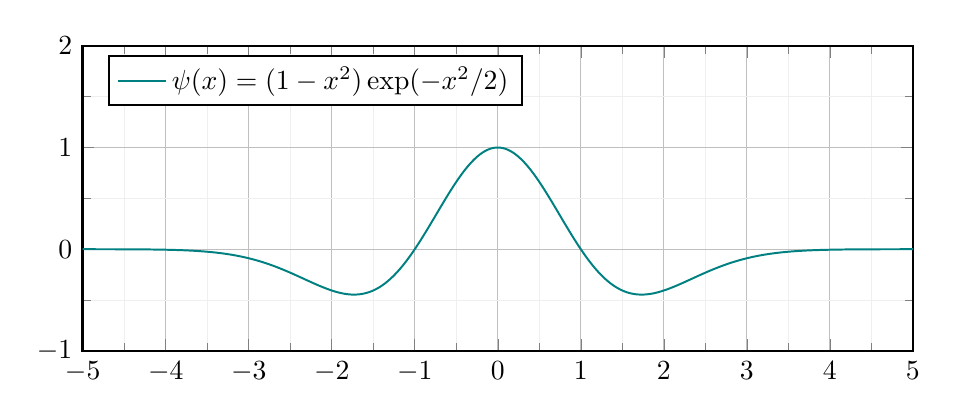
\begin{tikzpicture}
		\begin{axis}[
			grid = both,
			legend pos = north west,
			minor tick num = 1,
			major grid style = {lightgray},
			minor grid style = {lightgray!25},
			width = \textwidth,
			height = 0.45 \textwidth,
			xmin=-5, xmax=5,
			ymin=-1, ymax=2,
			line width=0.3mm
			]
			
			\addplot[domain = -5:5,
			samples = 300,
			color = teal,
			smooth,
			line width = 0.025cm,] {(1 - x^2) * exp(-(x^2) / 2)};
			
			\legend{$\psi(x) = (1 - x^2)\exp(-x^2/2)$};
		\end{axis}
	\end{tikzpicture}
	\caption{Иллюстрация wavelet <<Мексиканская шляпа>>}
	\label{pic::mexican_hat_wavelet}
\end{figure}
\noindent Сама по себе архитектура данной сети сходится к построению однослойной сети, на вход которой подается временной ряд, а на выход получается одно число, сформированное посредством параллельного воздействия всех wavelon'ов на величины имеющегося сигнала. Соответственно, выражаем данную самообучающуюся функцию через аналитическую запись, взятую из \cite{alexandridis2014wavelet}.
\begin{equation}
	f(x) \equiv g_{k}(x, \hat{w}_n) = \overbrace{w_{k + 1}^{[2]} + \sum_{i = 1}^m w_i^{[0]} \cdot x_{i}}^{\text{Линейная модель}} + \overbrace{\sum_{j = 1}^k w_{j}^{[2]} \cdot \prod_{i = 1}^{m} \psi\left(\frac{x_i - w_{ij}^{t}}{w_{ij}^{d}}\right)}^{\text{Wavelet модель}}
\end{equation}
\noindent Где $x \in \R^m, \hat{w}_n \in \R^{m \times k}, \hat{w} = \left\{ w_{i}^{[0]}, w_{j}^{[2]}, w_{k + 1}^{[2]}, w_{ij}^t, w_{ij}^d \right\}$ --- настраиваемые в процессе обучения параметры. Линейная модель включена сюда для наличия прямой связи того, что было, с тем, что прогнозируется. Далее рассматриваем пример работы описанной модели на имеющихся данных о ценах открытия компании Ford.

Для начала смотрим на графики поведения функционала потерь и функции метрики для цен компании:
\begin{figure}[H]
	\centering
	\includegraphics[width= 15cm]{nn/wn/ford_train_val_prices.png}
	\caption{График MSE для Wavelet Network (цены USD)}
	\label{fig::wn_ford_train_val_prices}
\end{figure}
\noindent Значения ведут себя достаточно <<красиво>>, что позволяет говорить о некоторой гладкости той поверхности, по которой скатывается градиент функции потерь. Данный факт обосновывается наличием работ, посвященных сходимости исследуемой сети \cite{alexandridis2014wavelet, zhang1992wavelet}, что дает преимущество настоящей сети перед классом Neural Network, для которых нет общего утверждения о сходимости к требуемым значениям. Теперь, исходя из аналогии предыдущих примеров, анализируем поведение лучшей валидационной метрики:
\begin{figure}[H]
	\centering
	\includegraphics[width= 17cm]{nn/wn/ford_best_metric_prices.png}
	\caption{График изменения лучшей валидационной метрики: WAPE}
	\label{fig::wn_ford_best_metric_prices}
\end{figure}
\noindent Она убывает также гладко, как и функции ошибок, что не может не радовать. В заключение работы с ценами, смотрим на предсказания:
\begin{figure}[H]
	\centering
	\includegraphics[width= 17cm]{nn/wn/ford_test_prices.png}
	\caption{График реальных и предсказанных цен акций Ford (USD)}
	\label{fig::wn_ford_test_prices}
\end{figure}
\noindent Результат превосходит блок Simple Recurrent Unit ($0.5$ USD), являвшимся лучшим среди всех примеров. Таким образом, данная сеть, исходя из проанализированных данных, лучше описывает их, чем ранее проверенная модель класса RNN. Аналогичный анализ проводим для доходностей.
\begin{figure}[H]
	\centering
	\includegraphics[width= 17cm]{nn/wn/ford_train_val_returns.png}
	\caption{График MSE для Wavelet Network (доходности \%)}
	\label{fig::wn_ford_train_val_returns}
\end{figure}
\noindent Поведение графиков такое же гладкое, как и для цен, однако выход на плато происходит быстрее, что, скорее всего, находит свое отражение в способности модели к прогнозированию доходностей. Смотрим на лучшую валидационную метрику:
\begin{figure}[H]
	\centering
	\includegraphics[width= 17cm]{nn/wn/ford_best_metric_returns.png}
	\caption{График изменения лучшей валидационной метрики: WAPE}
	\label{fig::wn_ford_best_metric_returns}
\end{figure}
\noindent Как и следовало ожидать, она достаточно гладкая. Но при этом аналогично функции метрики и функционала потерь для цен демонстрирует быстрый выход на плато. Далее --- анализируем полученные предсказания:
\begin{figure}[H]
	\centering
	\includegraphics[width= 17cm]{nn/wn/ford_test_returns.png}
	\caption{График реальных и предсказанных доходностей Ford (\%)}
	\label{fig::wn_ford_test_returns}
\end{figure} 
Удивительно, но при достаточно скромных предсказаниях --- очень близких к $0$ по сравнению со своими реальными значениями --- модель демонстрирует меньшую RMSE метрику, чем блок GRU ($2.89\%$), что наталкивает на мыль о большей пригодности данной модели к работе с доходностями. Однако, нет, отклонение опять больше, чем предсказанное значение, следовательно, использование полученных прогнозов на практике однозначно приводит к заблуждениям и некорректным выводам. Несмотря на все полученных негативные результаты при работе с доходностями, модель включается в финальную сравнительную таблицу как способная к прогнозированию. Но при этом не забываем, что важно учитывать особенности данных, на которых обучалась модель, ведь может оказаться, что меньшая ошибка на ценах и/или на доходностях --- случайный успех.

В заключении рассмотренного блока невозможно не сделать вывод, что все вышесказанное --- сложная математическая составляющая, призванная хотя бы немного описать реальные данные, содержащие поведение цены открытия акций и доходностей соответственно. Безусловно это сложно, а, придерживаясь гипотезы эффективного рынка, вообще невозможно. Поэтому замечаем, что настоящая работа не призвана создавать что-то новое. Она носит характер выбора из уже имеющегося, то есть --- последовательный сравнительный анализ моделей на данных 15 компаний развитого (US) и развивающегося (Китай) рынков на основе метрической функции Weighted Average Percentage Error (WAPE). В итоге получаем набор метрических характеристик типа: Тип рынка; Компания; Исследуемый объект (цена или доходность); значение WAPE.

В следующих блоках более детально рассматриваем как каждый из указанных рынков, так и сам по себе эксперимент. После чего интерпретируем полученные результаты и делаем выводы, основываясь на них.